\section{常见的并行模式}
当我们作为程序员处于最佳状态时,我们会认识到工作中的模式并应用经过时间考验的最佳解决方案技术。 
并行编程也不例外,如果不研究已被证明在该领域有用的模式,那将是一个严重的错误。 
考虑大数据应用程序采用的 MapReduce 框架; 他们的成功很大程度上源于基于两种简单而有效的并行模式——映射和归约。

并行编程中有许多常见的模式,它们会一次又一次地出现,与我们使用的编程语言无关。 
这些模式用途广泛,可以在任何并行级别(例如Sub-Groups、Work-Groups、完整设备)和任何设备(例如 CPU、GPU、FPGA)上使用。 
然而,模式的某些属性(例如它们的可扩展性)可能会影响它们对不同设备的适用性。 
在某些情况下,使应用程序适应新设备可能只需要选择适当的参数或微调模式的实现; 
在其他情况下,我们也许能够通过选择完全不同的模式来提高性能。

了解如何、何时、何地使用这些常见并行模式是提高 SYCL(以及一般并行编程)熟练程度的关键部分。 
对于那些具有现有并行编程经验的人来说,了解这些模式在 SYCL 中的表达方式可以是快速启动并熟悉该语言功能的方法。

本章旨在回答以下问题:

\begin{itemize}
	\item 我们应该了解哪些常见模式?

	\item 这些模式与不同设备的功能有何关系?

	\item 哪些模式已作为 SYCL 函数和库提供?

	\item 如何使用直接编程来实现这些模式?
\end{itemize}


\subsection{理解模式}
这里讨论的模式是 McCool 等人的《结构化并行编程》一书中描述的并行模式的子集。 
我们不讨论与并行类型相关的模式(例如,fork-join、branch-and-bound),
而是关注一些对于编写数据并行Kernel最有用的算法模式。

\begin{figure}[H]
	\centering
	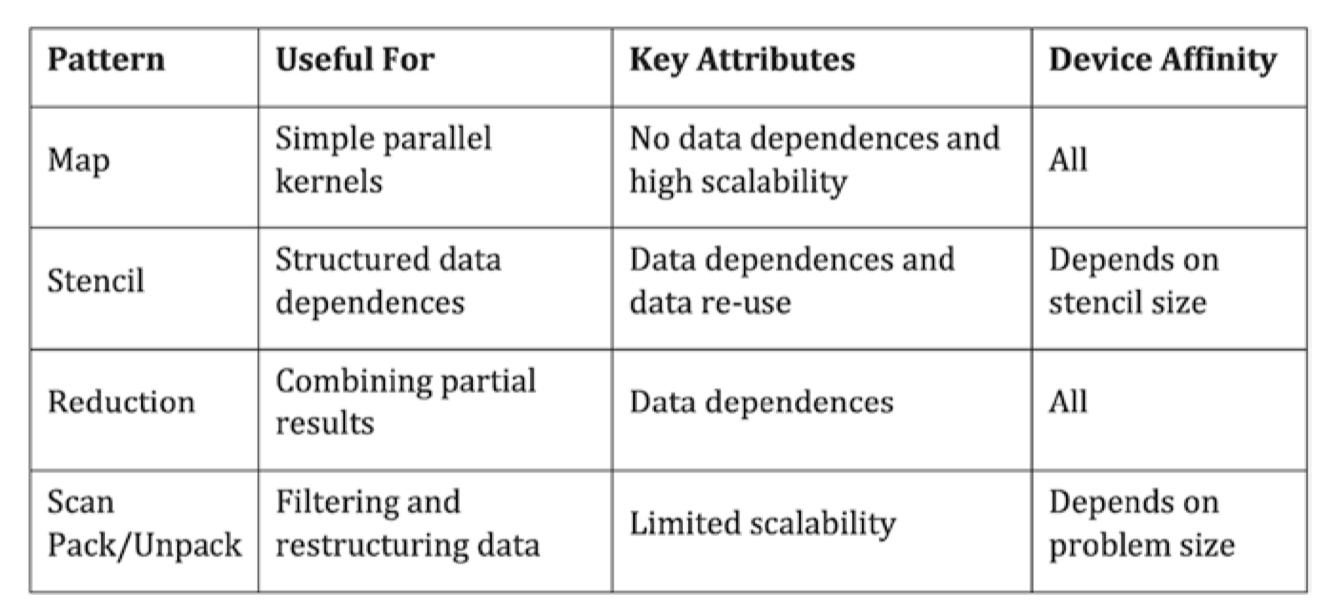
\includegraphics[width=0.9\textwidth]{figs/F14.1.png}
	\caption{\textit{并行模式及其对不同设备类型的亲和力 }}
\end{figure}

我们全心全意地相信,理解并行模式的这个子集对于成为一名有效的 SYCL 程序员至关重要。 
图 14-1 中的表提供了不同模式的高级概述,
包括它们的主要用例、关键属性以及它们的属性如何影响它们对不同硬件设备的亲和力。

\subsubsection{映射 Map}
\begin{figure}[H]
	\centering
	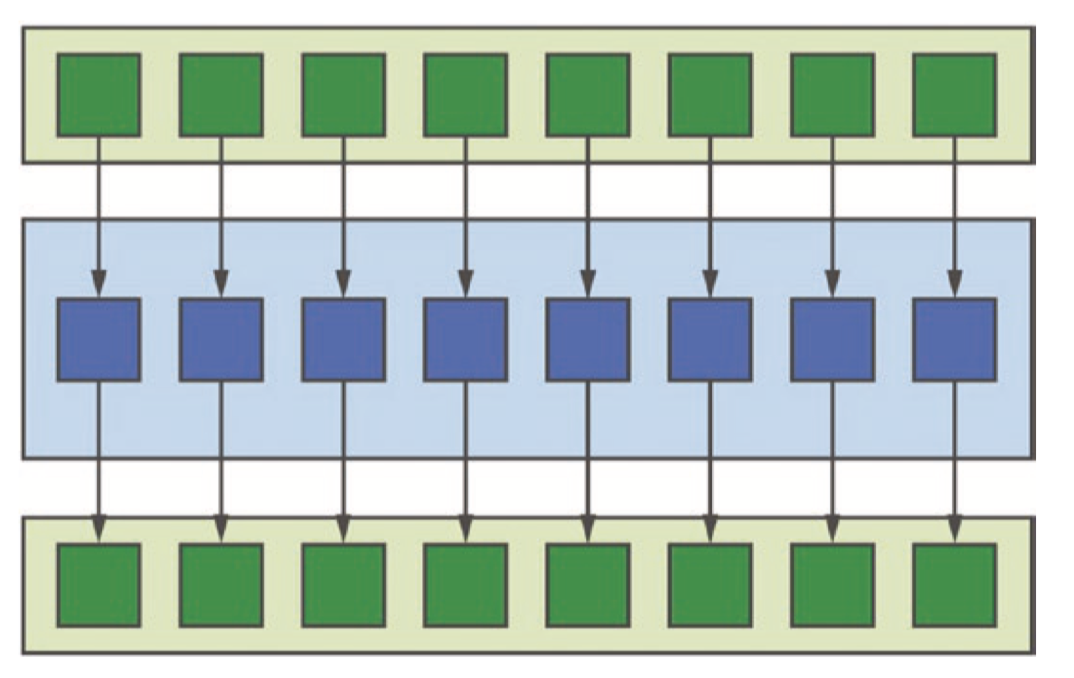
\includegraphics[width=0.9\textwidth]{figs/F14.2.png}
	\caption{\textit{Map 模式 }}
\end{figure}

映射模式是所有并行模式中最简单的,具有函数式编程语言经验的读者会立即熟悉。 
如图 14-2 所示,范围的每个输入元素通过应用某种函数独立地映射到输出。 
许多数据并行操作可以表示为映射模式的实例(例如,向量加法)。

由于函数的每个应用程序都是完全独立的,因此映射的表达式通常非常简单,依赖于编译器和/或运行时来完成大部分艰苦的工作。 
我们应该期望写入映射模式的Kernel适用于任何设备,并且这些Kernel的性能能够随着可用硬件并行性的数量很好地扩展。

然而,在决定将整个应用程序重写为一系列映射Kernel之前,我们应该仔细考虑! 
这种开发方法效率很高,并保证应用程序可以移植到各种设备类型,
但鼓励我们忽略可能显着提高性能的优化(例如,提高数据重用、融合Kernel)。

\subsubsection{模版 Stencil}
\begin{figure}[H]
	\centering
	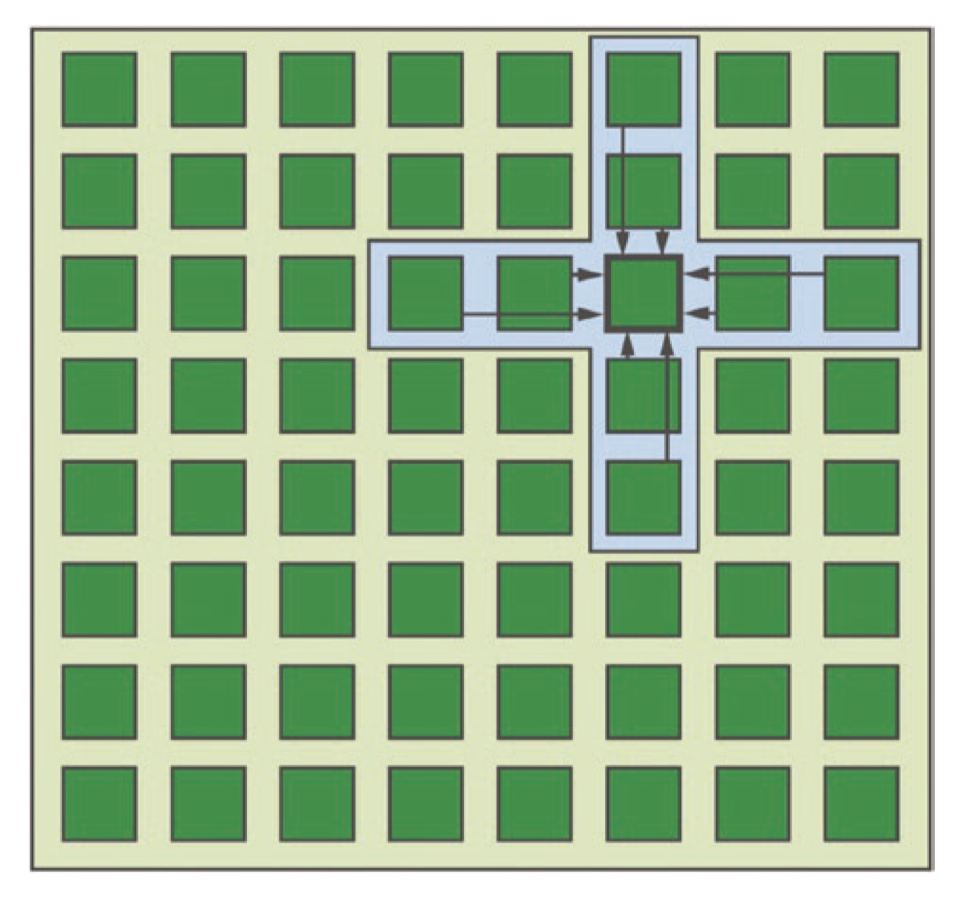
\includegraphics[width=0.9\textwidth]{figs/F14.3.png}
	\caption{\textit{Stencil 模式 }}
\end{figure}

模板模式与映射模式密切相关。 如图 14-3 所示,将一个函数应用于一个输入和由模板描述的一组相邻输入以产生单个输出。 
模板模式经常出现在许多领域,包括科学/工程应用(例如,有限差分代码)和计算机视觉/机器学习应用(例如,图像卷积)。

当模板模式异位执行时(即,将输出写入单独的存储位置),该函数可以独立应用于每个输入。 
在现实世界中调度模板通常比这更复杂:计算相邻输出需要相同的数据,并且多次从内存加载该数据会降低性能; 
我们可能希望就地应用模板(即覆盖原始输入值),以减少应用程序的内存占用。

因此,模板Kernel对不同设备的适用性很大程度上取决于模板的属性和输入问题。 一般来说,

\begin{itemize}
	\item 小型模板可以受益于GPU 的暂存器存储。

	\item 大型模板可以受益于(相对)较大的CPU 缓存。

	\item 在小输入上运行的小型模板可以通过在 FPGA 上作为脉动阵列实现来实现显着的性能增益。
\end{itemize}

由于模板很容易描述,但有效实现却很复杂,因此许多模板应用程序都使用特定于域的语言 (DSL)。 
已经有一些嵌入式 DSL 利用 C++ 的模板元编程功能在编译时生成高性能模板Kernel。

\subsubsection{归约 Reduction}
归约是一种常见的并行模式,它使用通常是关联和交换的运算符(例如加法)来组合部分结果。 
最常见的归约示例是计算总和(例如,在计算点积时)或计算最小值/最大值(例如,使用最大速度来设置时间步长)。

\begin{figure}[H]
	\centering
	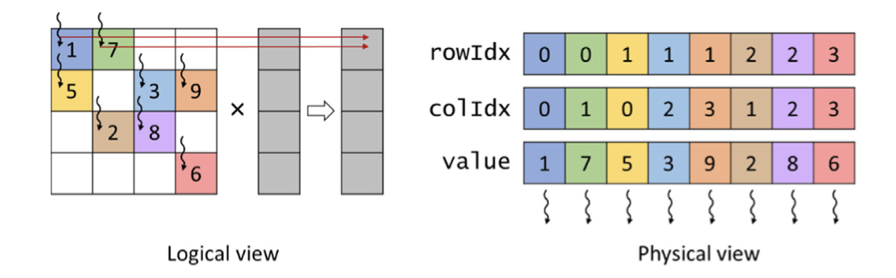
\includegraphics[width=0.9\textwidth]{figs/F14.4.png}
	\caption{\textit{Reduction 模式 }}
\end{figure}

图 14-4 显示了通过树归约实现的归约模式,这是一种流行的实现,需要对一系列 N 个输入元素进行 log2 (N) 组合操作。 
尽管树归约很常见,但其他实现也是可能的 - 一般来说,我们不应该假设归约按特定顺序组合值。

在现实生活中,Kernel很少是令人尴尬的并行,即使是这样,它们也经常与归约(如在 MapReduce 框架中)配对来总结其结果。 
这使得归约成为需要理解的最重要的并行模式之一,并且我们必须能够在任何设备上高效执行该模式。

调优不同设备的归约是计算部分结果所花费的时间和组合它们所花费的时间之间的微妙平衡行为; 
使用太少的并行性会增加计算时间,而使用太多的并行性会增加组合时间。

通过使用不同的设备来执行计算和组合步骤来提高整体系统利用率可能很诱人,
但这种调整工作必须仔细注意在设备之间移动数据的成本。 
在实践中,我们发现在同一设备上直接对生成的数据进行归约通常是最好的方法。 
因此,使用多个设备来提高归约模式的性能并不依赖于任务并行性,
而是依赖于另一个级别的数据并行性(即,每个设备对部分输入数据执行归约)。

\subsubsection{扫描 Scan}
扫描模式使用二元关联运算符计算广义前缀和,并且输出的每个元素代表部分结果。 
如果元素 i 的部分和是范围 [0, i] 中所有元素的总和(即包括 i 的总和),则称扫描是包含的。 
如果元素 i 的部分和是 [0, i) 范围内所有元素的和(即不包括 i 的和),则称扫描是排他的。

乍一看,扫描似乎是一种本质上的串行操作——每个输出的值取决于前一个输出的值! 
虽然扫描确实比其他模式具有更少的并行机会(因此可扩展性可能较差),
但图 14-5 表明可以使用对相同数据的多次扫描来实现并行扫描。

\begin{figure}[H]
	\centering
	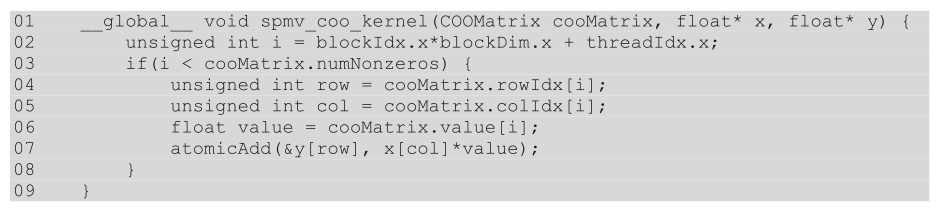
\includegraphics[width=0.9\textwidth]{figs/F14.5.png}
	\caption{\textit{Scan 模式 }}
\end{figure}

由于扫描操作中并行性的机会有限,因此执行扫描的最佳设备高度依赖于问题大小:较小的问题更适合 CPU,
因为只有较大的问题才会包含足够的数据并行性来饱和 图形处理器。 
对于 FPGA 和其他空间架构来说,问题大小不太重要,因为扫描自然适合管道并行性。 
与归约的情况一样,在生成数据的同一设备上执行扫描操作通常是一个好主意,
考虑到优化期间扫描操作在何处以及如何适应应用程序,通常会比专注于优化数据产生更好的结果。 隔离扫描操作。

\subsubsection{打包和拆包}
打包和解包模式与扫描密切相关,并且通常在扫描功能之上实现。 
我们在这里单独介绍它们,因为它们可以实现常见操作(例如附加到列表)的高性能实现,
而这些操作可能与前缀和没有明显的联系。

\paragraph{打包 Pack}

\begin{figure}[H]
	\centering
	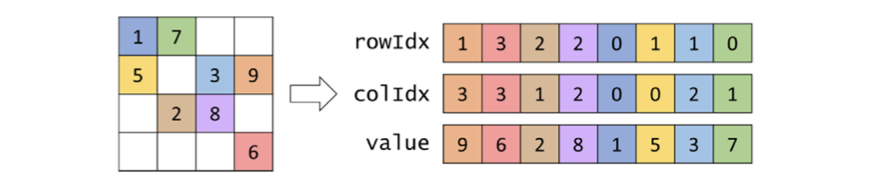
\includegraphics[width=0.9\textwidth]{figs/F14.6.png}
	\caption{\textit{Pack 模式 }}
\end{figure}

如图 14-6 所示,打包模式根据布尔条件丢弃输入范围的元素,将未丢弃的元素打包到输出范围的连续位置。 
该布尔条件可以是预先计算的掩码,也可以通过对每个输入元素应用某些函数来在线计算。

与扫描一样,打包操作具有固有的串行性质。 给定要打包/复制的输入元素,
计算其在输出范围中的位置需要有关有多少先前元素也被打包/复制到输出中的信息。 
该信息相当于对驱动包的布尔条件进行独占扫描。

\paragraph{拆包 Unpack}

\begin{figure}[H]
	\centering
	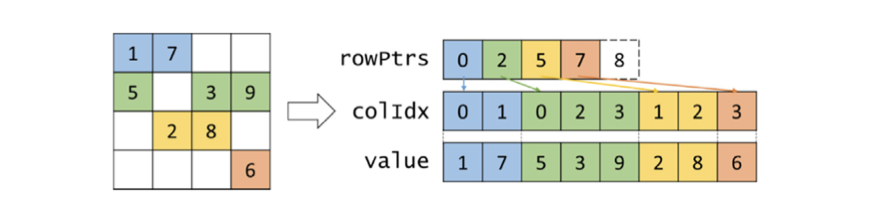
\includegraphics[width=0.9\textwidth]{figs/F14.7.png}
	\caption{\textit{Unpack 模式 }}
\end{figure}

如图 14-7 所示(顾名思义),解包模式与打包模式相反。 
输入范围的连续元素被解包为输出范围的不连续元素,而其他元素保持不变。 
此模式最明显的用例是解压缩先前打包的数据,但它也可用于填充先前计算产生的数据中的“间隙”。

\subsection{使用内置函数和库}
其中许多模式可以使用 SYCL 的内置功能或供应商提供的用 SYCL 编写的库直接表达。 
利用这些函数和库是在真正的大型软件工程项目中平衡性能、可移植性和生产力的最佳方式。

\subsubsection{SYCL 归约库}
SYCL 不需要我们每个人都维护自己的可移植且高性能的归约Kernel库,
而是提供了一种方便的抽象,用于使用归约语义来描述变量。 
这种抽象简化了约简Kernel的表达,并使约简的执行变得明确,
允许实现针对设备、数据类型和约简操作的不同组合在不同的约简算法之间进行选择。

\begin{figure}[H]
	\centering
	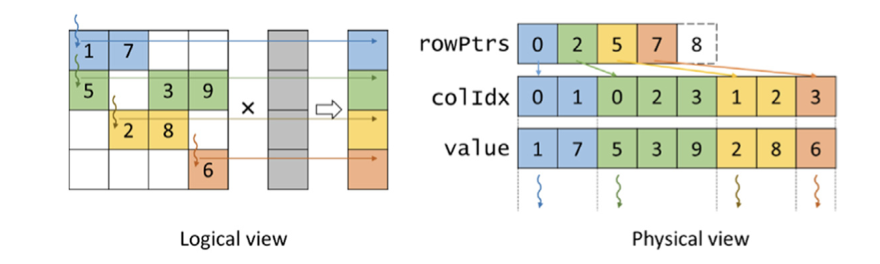
\includegraphics[width=0.9\textwidth]{figs/F14.8.png}
	\caption{\textit{使用 reduction 库表示为数据并行Kernel的 Reduction }}
\end{figure}

图 14-8 中的Kernel显示了使用归约库的示例。 
请注意,Kernel主体不包含任何对归约的引用 - 我们必须指定的是Kernel包含使用加函Sub-Groups合 sum 变量实例的归约。 
这为实现自动生成优化的归约序列提供了足够的信息。

在Kernel完成之前,不能保证归约结果被写回原始变量。 
除了此限制之外,访问归约结果的行为与访问 SYCL 中任何其他变量的行为相同:
访问存储在缓冲区中的归约结果需要创建适当的设备或主机访问器,
并且访问存储在 USM 分配中的归约结果 可能需要显式同步和/或内存移动。

SYCL 归约库与其他语言中的归约抽象不同的一个重要方式是,
它限制我们在Kernel执行期间对归约变量的访问 - 我们无法检查归约变量的中间值,
并且禁止更新归约变量 使用指定组合函数以外的任何变量。 
这些限制可以防止我们犯下难以调试的错误(例如,在尝试计算最大值时添加归约变量),
并确保可以在各种不同的设备上有效地实现归约。

\paragraph{reduction 类}

\begin{figure}[H]
	\centering
	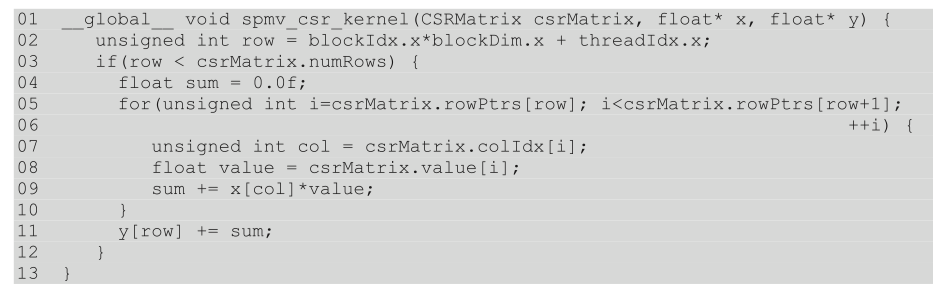
\includegraphics[width=0.9\textwidth]{figs/F14.9.png}
	\caption{\textit{a }}
\end{figure}

归约类是我们用来描述Kernel中存在的归约的接口。 构造归约对象的唯一方法是使用图 14-9 中所示的函数之一。 
请注意,共有三个归约函数系列(用于缓冲区、USM 指针和跨度),每个系列都有两个重载(带和不带恒等变量)。

如果使用缓冲区或 USM 指针初始化归约,则归约是标量归约,对数组中的第一个对象进行操作。 
如果使用跨度初始化归约,则归约是数组归约。 
数组归约的每个组成部分都是独立的——我们可以认为对大小为 N 的数组进行数组归约操作
相当于具有相同数据类型和运算符的 N 标量归约。

该函数最简单的重载允许我们指定归约变量和用于组合每个Work-Items的贡献的运算符。 
第二组重载允许我们提供与归约运算符关联的可选标识值 - 这是对用户定义归约的优化,我们稍后将重新讨论。

请注意,归约函数的返回类型是未指定的,并且归约类本身完全是实现定义的。 
尽管这对于 C++ 类来说可能有点不寻常,
但它允许实现使用不同的类(或具有任意数量的模板参数的单个类)来表示不同的归约算法。 
SYCL 的未来版本可能会决定重新审视此设计,
以便使我们能够在特定执行上下文中显式请求特定的归约算法(最有可能通过 property\_list 参数)。

\paragraph{reducer 类}

\begin{figure}[H]
	\centering
	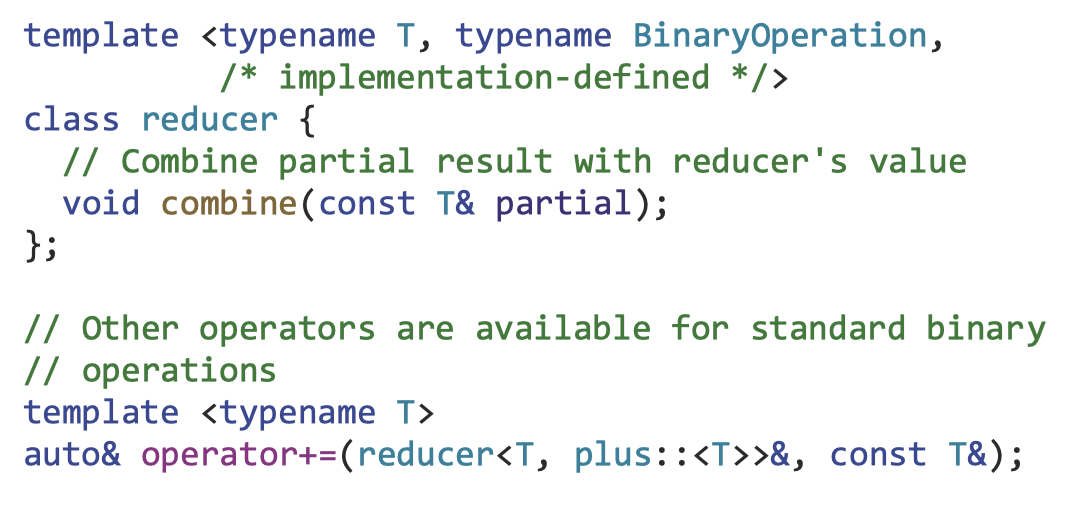
\includegraphics[width=0.9\textwidth]{figs/F14.10.png}
	\caption{\textit{reducer 类的简化定义 }}
\end{figure}

reducer 类的实例封装了一个归约变量,公开了一个有限的接口,确保我们无法以实现可能认为不安全的任何方式更新归约变量。 
reducer 类的简化定义如图 14-10 所示。

与归约类一样,归约器类的精确定义是实现定义的 - 归约器的类型将取决于归约的执行方式,
为了最大限度地提高性能,在编译时了解这一点非常重要。 
然而,允许我们更新归约变量的函数和运算符已明确定义,并且保证受到任何 SYCL 实现的支持。

具体来说,每个reducer 都提供一个combine() 函数,它将部分结果(来自单个Work-Items)与reduction 变量的值组合起来。 
这个组合函数的行为方式是实现定义的,但在编写Kernel时我们不需要担心。 
还需要一个reducer来根据reducer操作符来提供其他操作符; 
例如,+= 运算符被定义为加减法。 提供这些附加运算符只是为了方便程序员并提高可读性; 
在可用的情况下,这些运算符与直接调用combine() 具有相同的行为。

当处理数组约简时,reducer 提供了一个额外的下标运算符(即,operator[]),允许访问数组的各个元素。 
该运算符不是直接返回对数组元素的引用,而是返回另一个化简器对象,
该对象公开与标量约简关联的约简器相同的 merge() 函数和简写运算符。 
图 14-11 显示了一个使用数组归约来计算直方图的Kernel的简单示例,其中下标运算符用于仅访问由Work-Items更新的直方图箱。

\begin{figure}[H]
	\centering
	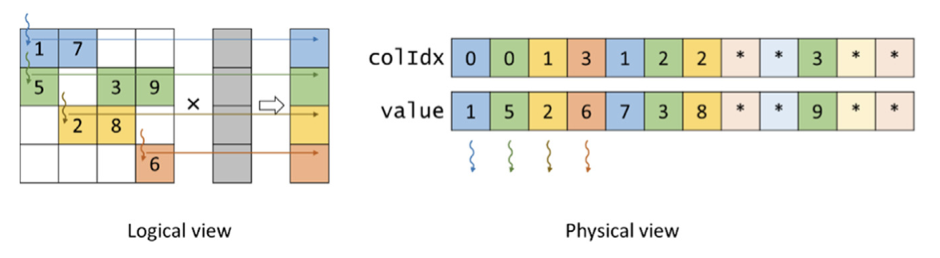
\includegraphics[width=0.9\textwidth]{figs/F14.11.png}
	\caption{\textit{使用数组约简计算直方图的示例Kernel }}
\end{figure}

\paragraph{用户定义的归约}

几种常见的归约算法(例如,树归约)不会看到每个Work-Items直接更新单个共享变量,
而是将一些部分结果累积在私有变量中,该变量将在将来的某个时刻进行组合。 
这样的私有变量引入了一个问题:实现应该如何初始化它们? 
将变量初始化为每个Work-Items的第一个贡献具有潜在的性能影响,因为需要额外的逻辑来检测和处理未初始化的变量。 
相反,将变量初始化为归约运算符的身份可以避免性能损失,但只有在身份已知的情况下才可能实现。

仅当对简单算术类型进行归约操作并且归约运算符是几个标准函数对象(例如,加号)之一时,
SYCL 实现才能自动确定要使用的正确标识值。 
对于用户定义的归约(即,对用户定义类型和/或使用用户定义函数对象进行操作的归约),我们可以通过直接指定标识值来提高性能。

对用户定义归约的支持仅限于可简单复制的类型和组合函数,
没有副作用,但这足以支持许多现实生活中的用例。 
例如,图 14-12 中的代码演示了如何使用用户定义的归约来计算向量中的最小元素及其位置。

\begin{figure}[H]
	\centering
	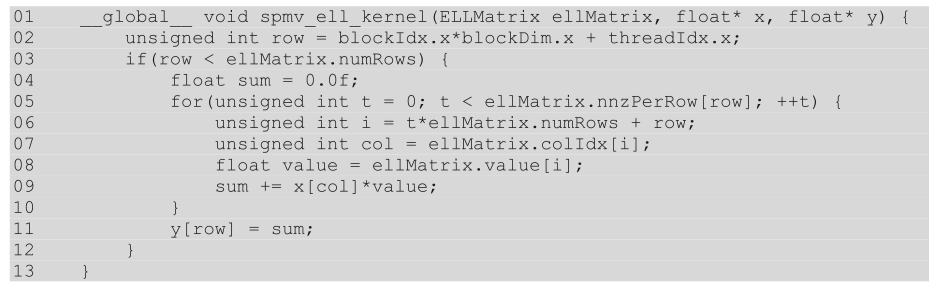
\includegraphics[width=0.9\textwidth]{figs/F14.12.png}
	\caption{\textit{使用用户定义的约简来查找最小值的位置 }}
\end{figure}

\subsubsection{集体算法}
SYCL 设备代码中对并行模式的支持由单独的组算法库提供。 
这些函数利用特定Work-Items组(即Work-Groups或Sub-Groups)的并行性在有限范围内实现常见并行算法,
并且可以用作构建其他更复杂算法的构建块。

SYCL 中的组算法的语法基于 C++ 中的算法库的语法,并且适用 C++ 算法的任何限制。 
然而,有一个关键的区别:STL 的算法是从顺序(主机)代码调用的,并表明库有机会采用并行性,
而 SYCL 的组算法则设计为在已经并行执行的(设备)代码内调用 。 
为了确保这种差异不会被忽视,组算法的语法和语义与其 C++ 对应算法略有不同。

SYCL 区分两种不同类型的并行算法。 如果一个算法由一个组中的所有Work-Items协作执行,
但在其他方面与 STL 中的算法行为相同,则该算法以“joint”前缀命名(因为该组的成员“joint”在一起执行该算法) )。 
此类算法从内存中读取输入并将结果写入内存,并且只能对给定组中的所有Work-Items可见的内存位置中的数据进行操作。 
如果算法在反映组本身的隐式范围内运行,
并且输入和输出存储在Work-Items私有内存中,
则算法名称将被修改为包含单词“组”(因为该算法直接对属于该组的数据执行) 团体)。

\begin{figure}[H]
	\centering
	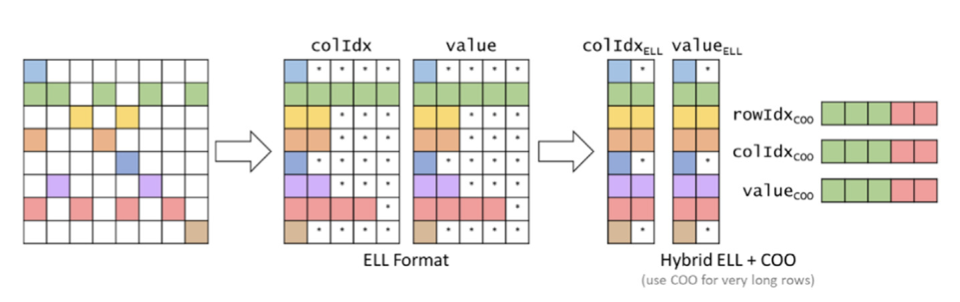
\includegraphics[width=0.9\textwidth]{figs/F14.13.png}
	\caption{\textit{std::reduce、sycl::joint\_reduce 和 sycl::reduce\_over\_group 的比较 }}
\end{figure}

图 14-13 中的代码示例演示了这两种不同类型的算法,
将 std::reduce 的行为与 sycl::joint\_reduce 和 sycl::reduce\_over\_group 的行为进行了比较。

请注意,在这两种情况下,每个组算法的第一个参数接受 group 或 sub\_group 对象来代替执行策略,
以描述应用于执行算法的Work-Items集。 
由于算法是由指定组中的所有Work-Items协同执行的,
因此它们也必须像组屏障一样对待——组中的所有Work-Items
必须在聚合控制流中遇到相同的算法(即,组中的所有Work-Items) 组必须类似地遇到或不遇到算法调用),
并且所有Work-Items提供的参数必须使得所有Work-Items都同意正在执行的操作。 
例如,sycl::joint\_reduce 要求所有Work-Items的所有参数都相同,
以确保组中的所有Work-Items对相同的数据进行操作并使用相同的运算符来累积结果。

\begin{figure}[H]
	\centering
	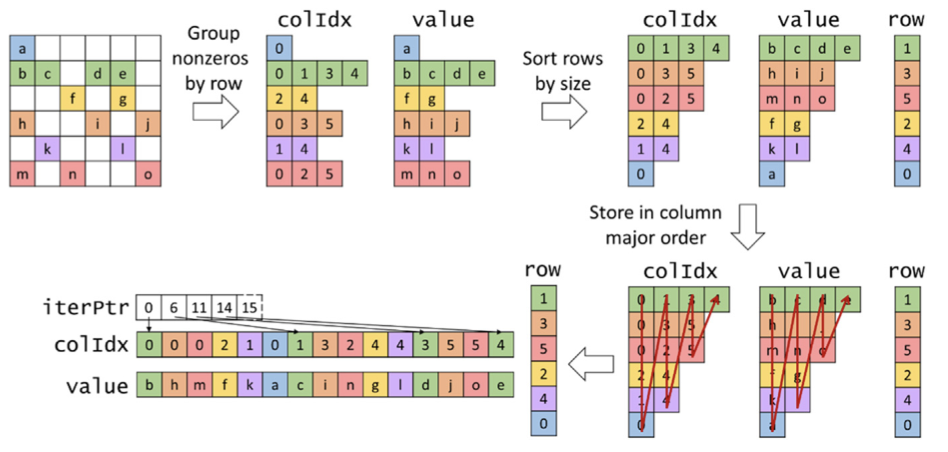
\includegraphics[width=0.9\textwidth]{figs/F14.14.png}
	\caption{\textit{C++ 算法和 SYCL 组算法之间的映射 }}
\end{figure}

图14-14中的表显示了STL中可用的并行算法与组算法的关系,以及对可以使用的组类型是否有任何限制。 
请注意,在某些情况下,组算法只能与Sub-Groups一起使用; 这些情况对应于前面章节中介绍的“shuffle”操作。

在撰写本文时,组算法仅限于支持基本数据类型和 SYCL 识别的一组内置运算符
(即plus, multiplies, bit\_and, bit\_or, bit\_xor, logical\_and, logical\_or, minimum, 和 maximum) 。 
这足以涵盖最常见的用例,但 SYCL 的未来版本预计将集体支持扩展到用户定义的类型和运算符。

\subsection{直接编程}
尽管我们建议尽可能利用库,但通过了解如何使用“本机”SYCL Kernel实现每种模式,我们可以学到很多东西。

本章剩余部分中的Kernel不应期望达到与高度调优的库相同的性能水平,
但有助于更好地理解 SYCL 的功能,甚至可以作为新库功能原型设计的起点 。

\begin{remark}[使用供应商提供的库!]
当供应商提供函数的库实现时,使用它几乎总是有益的,而不是将函数重新实现为Kernel!
\end{remark}

\subsubsection{映射 Map}
由于其简单性,映射模式可以直接实现为基本并行Kernel。 
图 14-15 中所示的代码显示了这样的实现,使用映射模式来计算范围内每个输入元素的平方根。

\begin{figure}[H]
	\centering
	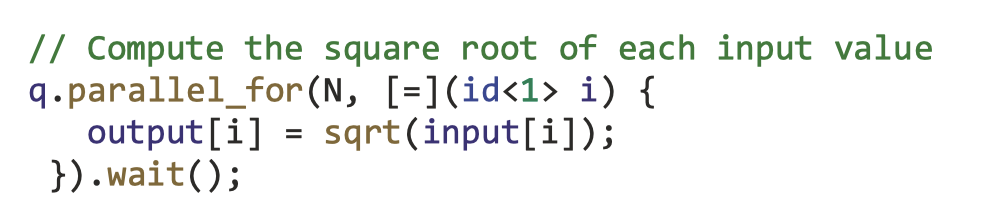
\includegraphics[width=0.9\textwidth]{figs/F14.15.png}
	\caption{\textit{在数据并行Kernel中实现Map模式 }}
\end{figure}

\subsubsection{模版 Stencil}
直接将模板实现为具有多维缓冲区的多维基本数据并行Kernel,如图 14-16 所示,非常简单且易于理解。

\begin{figure}[H]
	\centering
	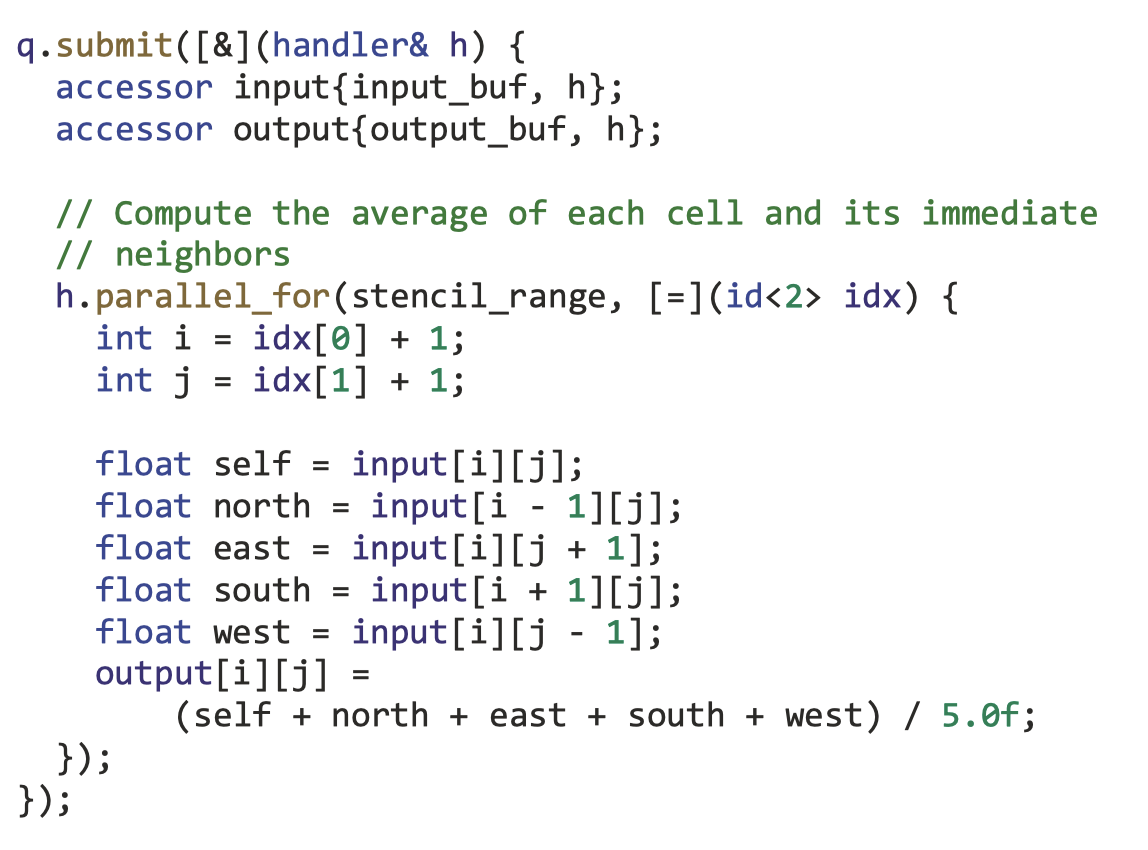
\includegraphics[width=0.9\textwidth]{figs/F14.16.png}
	\caption{\textit{在数据并行Kernel中实现 Stencil 模式 }}
\end{figure}

然而,这种模板模式的表达方式非常幼稚,不应期望表现得很好。 
正如本章前面提到的,众所周知,需要利用局部性(通过空间或时间阻塞)来避免从内存中重复读取相同的数据。 
图 14-17 显示了使用Work-Groups本地内存的空间阻塞的简单示例。

\begin{figure}[H]
	\centering
	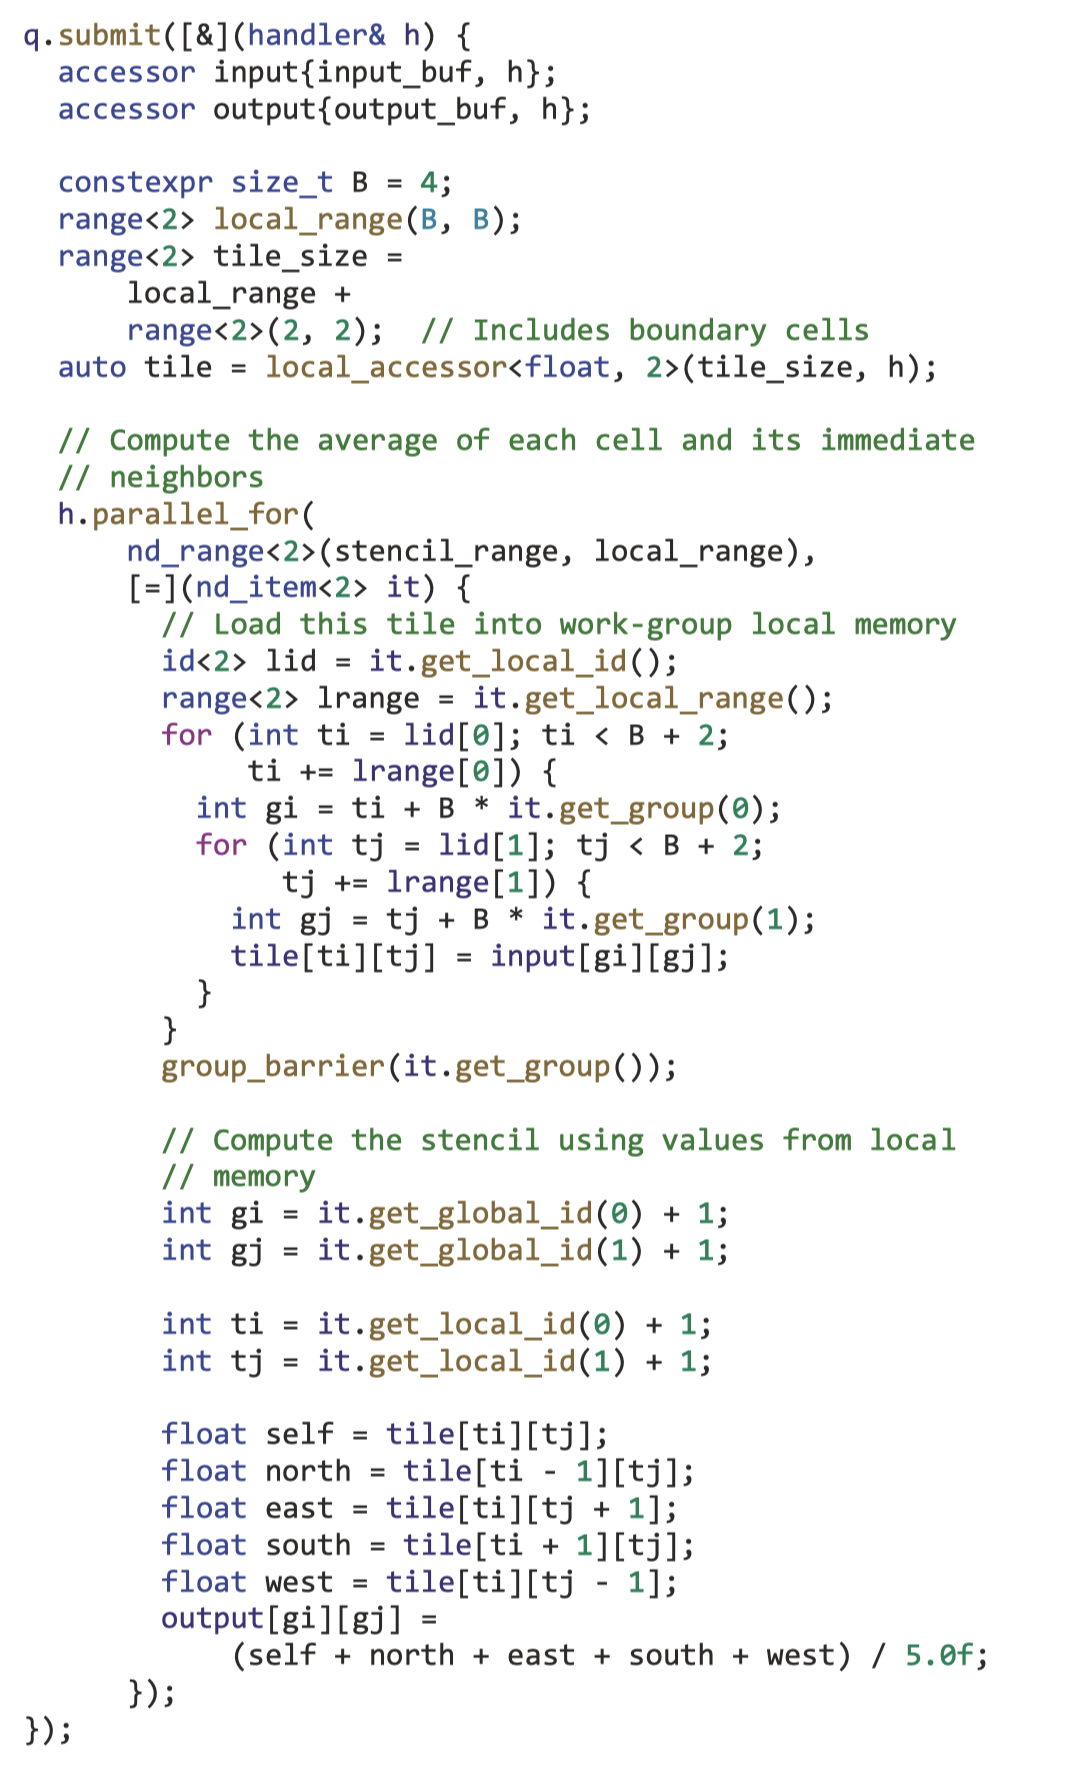
\includegraphics[width=0.9\textwidth]{figs/F14.17.png}
	\caption{\textit{使用Work-Groups本地内存在 ND 范围Kernel中实现 Stencil 模式 }}
\end{figure}

为给定模板选择最佳优化需要在编译时对块大小、邻域和模板函数本身进行自省,这需要比此处讨论的更复杂的方法。

\subsubsection{归约 Reduction}
\begin{figure}[H]
	\centering
	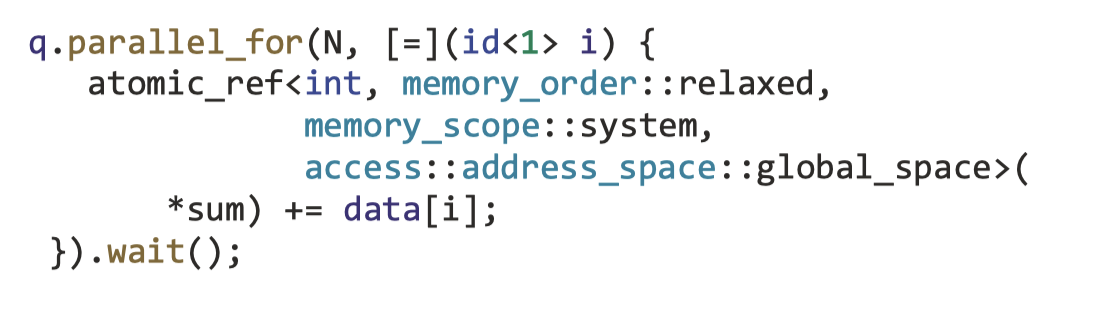
\includegraphics[width=0.9\textwidth]{figs/F14.18.png}
	\caption{\textit{实现以数据并行Kernel表示的朴素归约 }}
\end{figure}

\begin{figure}[H]
	\centering
	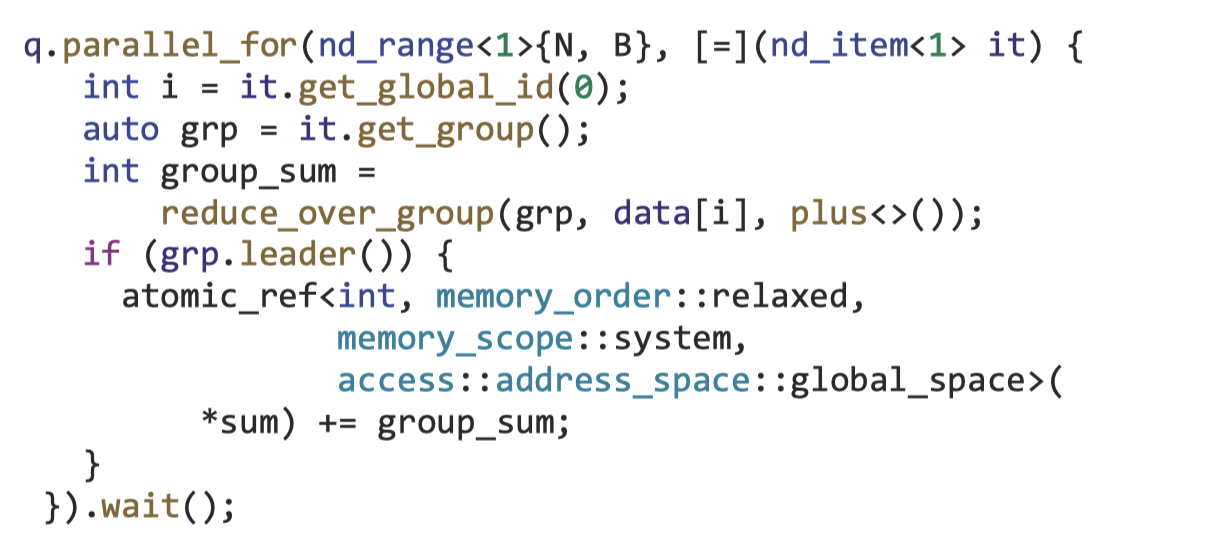
\includegraphics[width=0.9\textwidth]{figs/F14.19.png}
	\caption{\textit{实现以 ND 范围Kernel表示的朴素归约 }}
\end{figure}

通过利用提供Work-Items之间的同步和通信功能的语言功能
(例如原子操作、Work-Groups和Sub-Groups功能、Sub-Groups“洗牌”),
可以在 SYCL 中实现归约Kernel。 
图 14-18 和图 14-19 中的Kernel显示了两种可能的归约实现:
使用基本的 parallel\_for 和每个Work-Items的原子操作的简单归约,
以及使用 ND 范围的 parallel\_for 和利用局部性的稍微聪明的归约。 
分别是Work-Groups归约功能。 我们将在第 19 章中更详细地回顾这些原子操作。

还有许多其他方法可以编写归约Kernel,并且由于原子操作的硬件支持、Work-Groups本地内存大小、
全局内存大小、快速设备范围屏障的可用性或 甚至可以使用专用的归约指令。 
在某些体系结构上,使用 log2 (N) 个单独的Kernel调用执行树归约甚至可能更快(或必要!)。

我们强烈建议仅在 SYCL 归约库不支持的情况下或在针对特定设备的功能微调Kernel时才应考虑手动实现归约,
即使如此,也只有在 100\% 确定 SYCL 的 内置归约表现不佳!

\subsubsection{扫描 Scan}
正如我们在本章前面所看到的,实现并行扫描需要对数据进行多次扫描,并且每次扫描之间发生同步。 
由于 SYCL 不提供同步 ND 范围内所有Work-Items的机制,
因此设备范围扫描的直接实现必须使用多个Kernel,这些Kernel通过全局内存传达部分结果。

\begin{figure}[H]
	\centering
	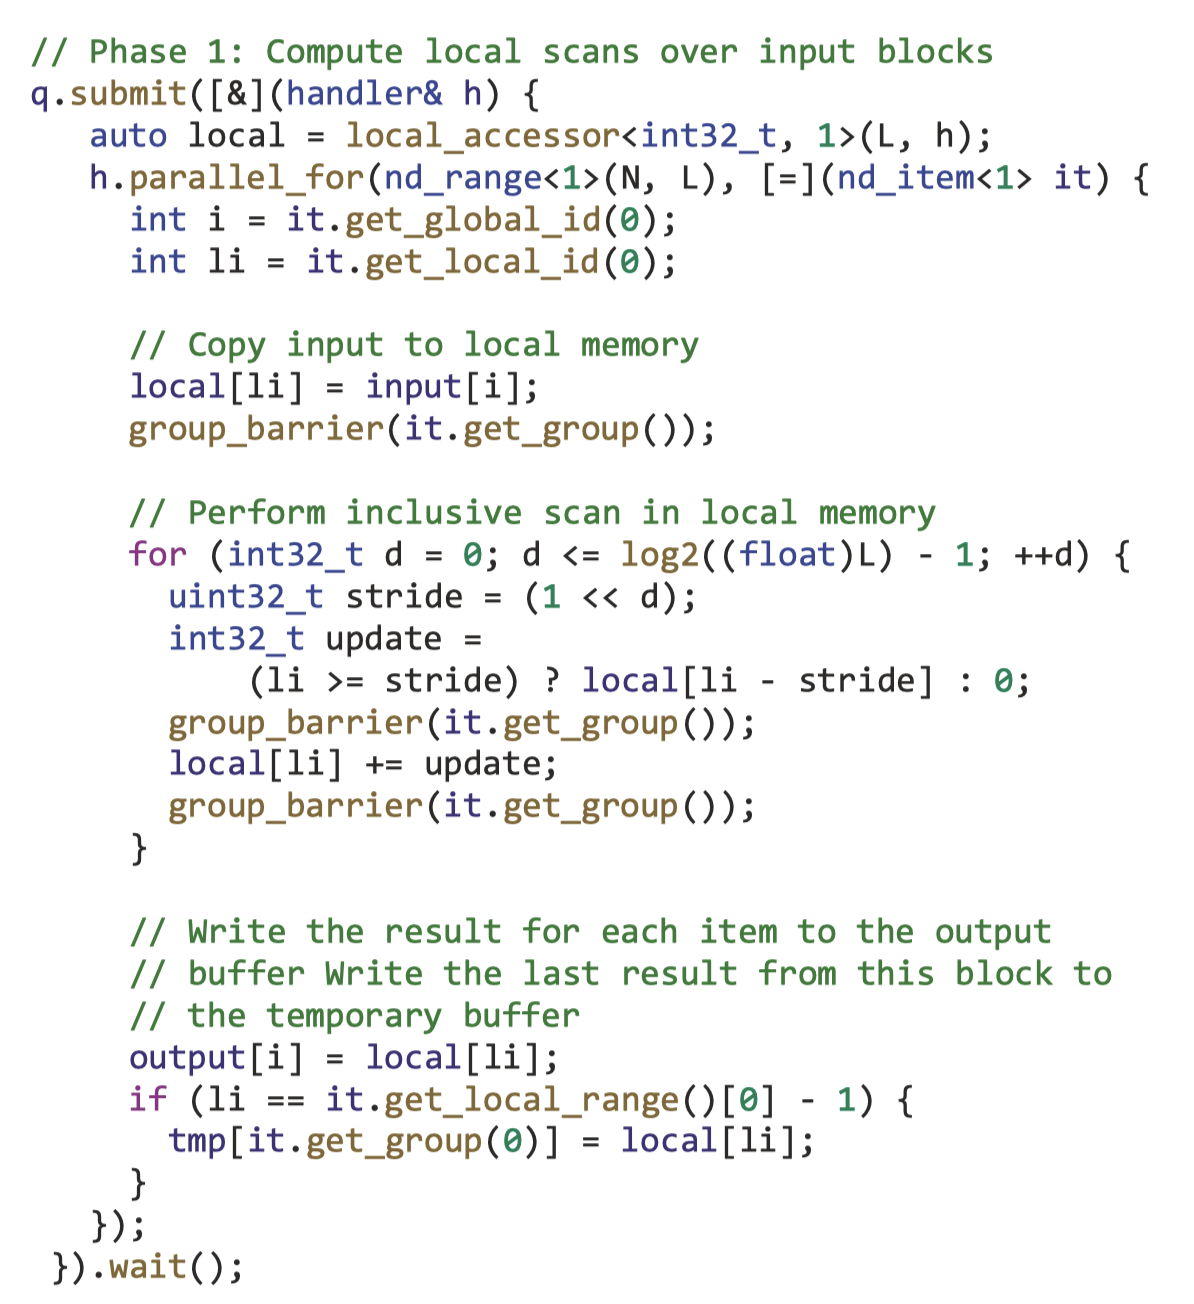
\includegraphics[width=0.9\textwidth]{figs/F14.20.png}
	\caption{\textit{在 ND 范围Kernel中实现全局包容性扫描的第 1 阶段:跨每个Work-Groups进行计算 }}
\end{figure}

\begin{figure}[H]
	\centering
	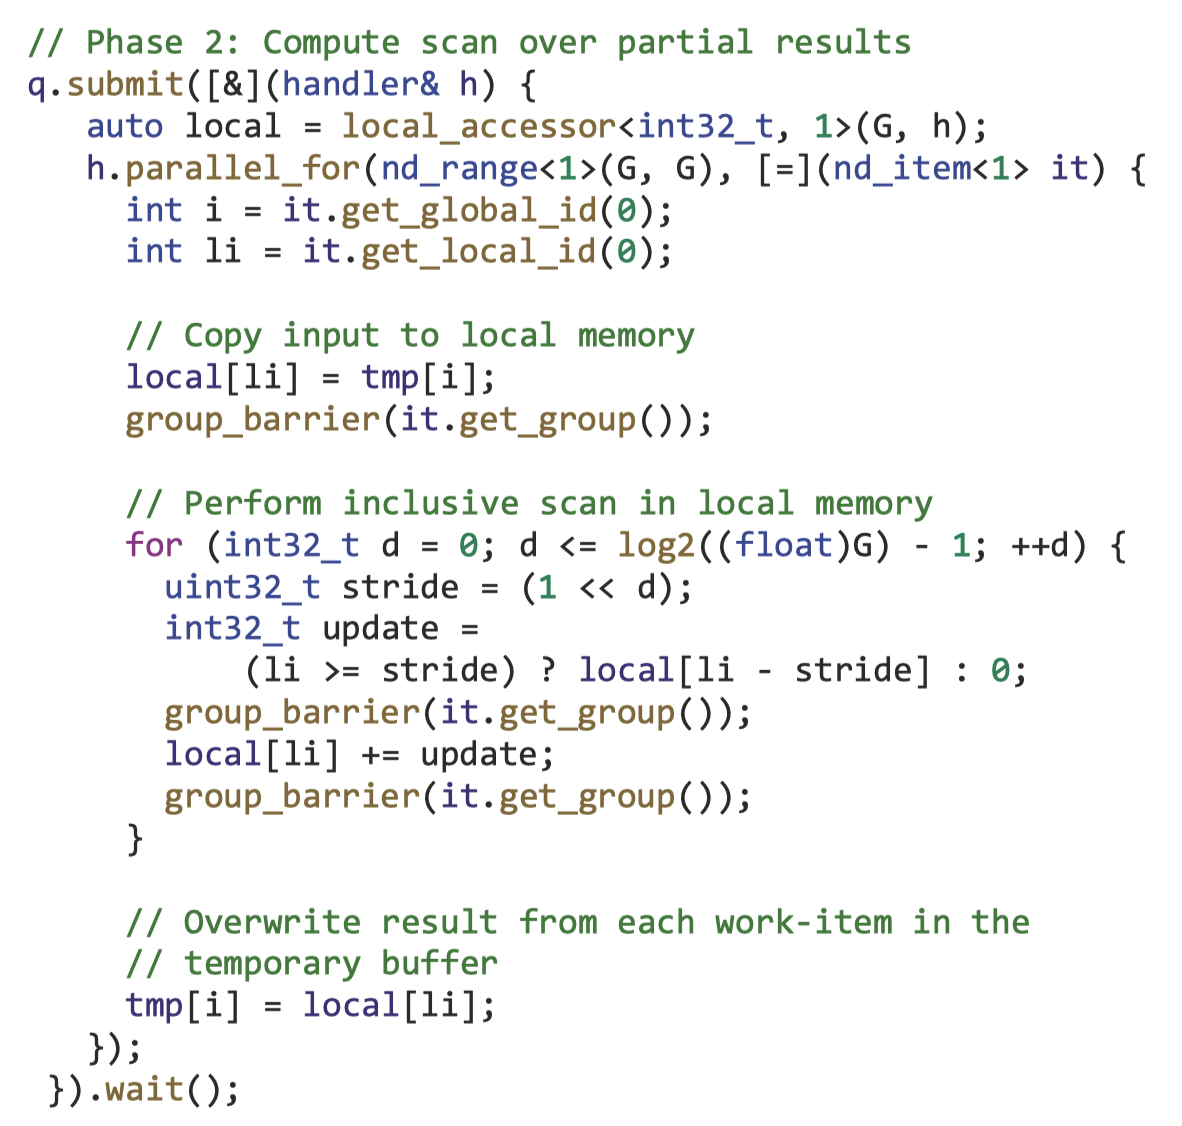
\includegraphics[width=0.9\textwidth]{figs/F14.21.png}
	\caption{\textit{在 ND 范围Kernel中实现全局包容性扫描的第 2 阶段:扫描每个Work-Groups的结果 }}
\end{figure}

\begin{figure}[H]
	\centering
	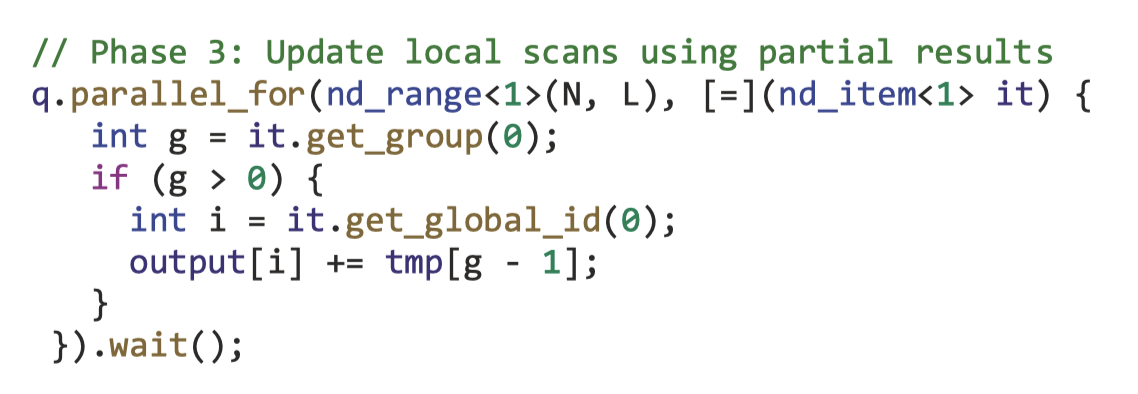
\includegraphics[width=0.9\textwidth]{figs/F14.22.png}
	\caption{\textit{第 3 阶段(最终阶段),用于在 ND 范围Kernel中实现全局包容性扫描 }}
\end{figure}

如图 14-20、14-21 和 14-22 所示的代码演示了使用多个Kernel实现的包含扫描。 
第一个Kernel将输入值分布在Work-Groups之间,
在Work-Groups本地内存中计算Work-Groups本地扫描(请注意,我们可以使用Work-Groups Include\_scan 函数来代替)。 
第二个Kernel使用单个Work-Groups计算本地扫描,这次是针对每个块的最终值。 
第三个Kernel结合这些中间结果来最终确定前缀和。 这三个Kernel对应于图 14-5 中的三层。

图14-20和图14-21非常相似; 唯一的区别是范围的大小以及输入和输出值的处理方式。 
此模式的实际实现可以使用采用不同参数的单个函数来实现这两个阶段,并且出于教学原因,它们仅在此处呈现为不同的代码。

\subsubsection{打包和拆包}
打包和解包也称为聚集和分散操作。 这些操作处理数据在内存中的排列方式以及我们希望如何将其呈现给计算资源的差异。

\paragraph{打包 Pack}

由于 pack 依赖于独占扫描,
因此实现适用于 ND 范围的所有元素的 pack 也必须通过全局内存并在多个Kernel队列的过程中进行。 
然而,pack 有一个常见的用例,不需要将操作应用于 ND 范围的所有元素,
即仅跨特定Work-Groups或Sub-Groups中的项目应用包。

\begin{figure}[H]
	\centering
	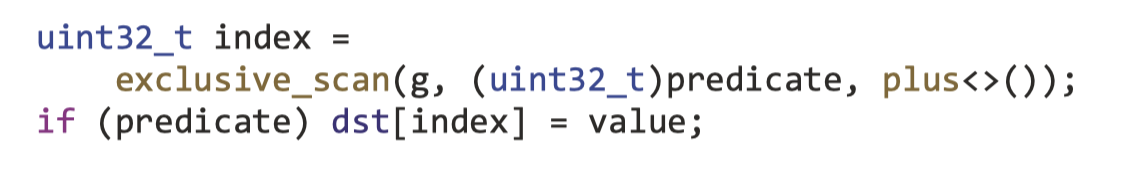
\includegraphics[width=0.9\textwidth]{figs/F14.23.png}
	\caption{\textit{在独占扫描之上实现组包操作 }}
\end{figure}

\begin{figure}[H]
	\centering
	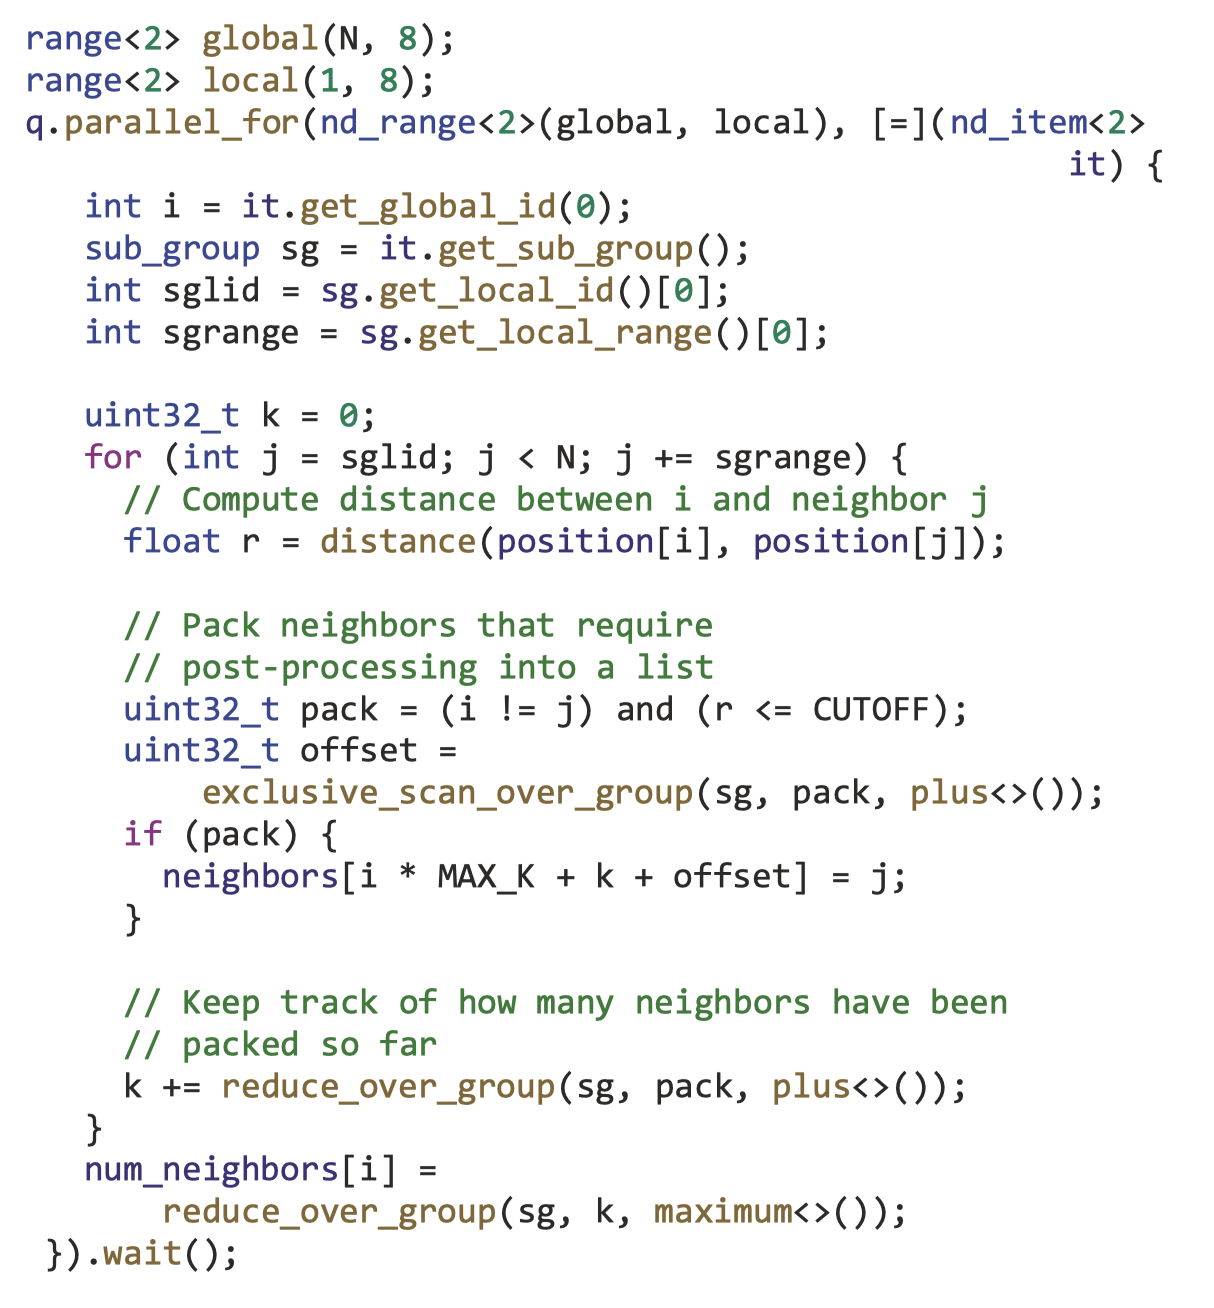
\includegraphics[width=0.9\textwidth]{figs/F14.24.png}
	\caption{\textit{使用Sub-Groups打包操作构建需要额外后处理的元素列表 }}
\end{figure}

图 14-23 中的代码片段展示了如何在独占扫描之上实现组包操作。

图 14-24 中的代码演示了如何在Kernel中使用此类打包操作来构建需要一些额外后处理(在未来的Kernel中)的元素列表。 
所示示例基于分子动力学模拟的真实Kernel:分配给粒子 i 的Sub-Groups中的Work-Items
合作识别 i 固定距离内的所有其他粒子,
并且仅识别此“邻居列表”中的粒子 将用于计算作用在每个粒子上的力。

请注意,打包模式永远不会对元素重新排序 - 打包到输出数组中的元素的显示顺序与输入中的顺序相同。 
pack 的这个属性很重要,
它使我们能够使用 pack 功能来实现其他更抽象的并行算法(例如 std::copy\_if 和 std::stable\_partition)。 
然而,还有其他并行算法可以在不需要维护顺序的包功能之上实现(例如 std::partition)。

\paragraph{拆包 Unpack}

\begin{figure}[H]
	\centering
	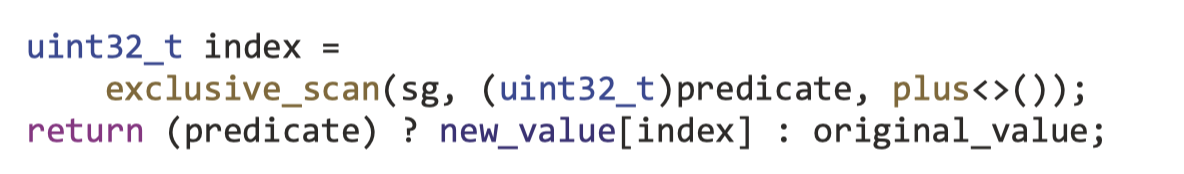
\includegraphics[width=0.9\textwidth]{figs/F14.25.png}
	\caption{\textit{在独占扫描之上实现Sub-Groups解压缩操作 }}
\end{figure}

\begin{figure}[H]
	\centering
	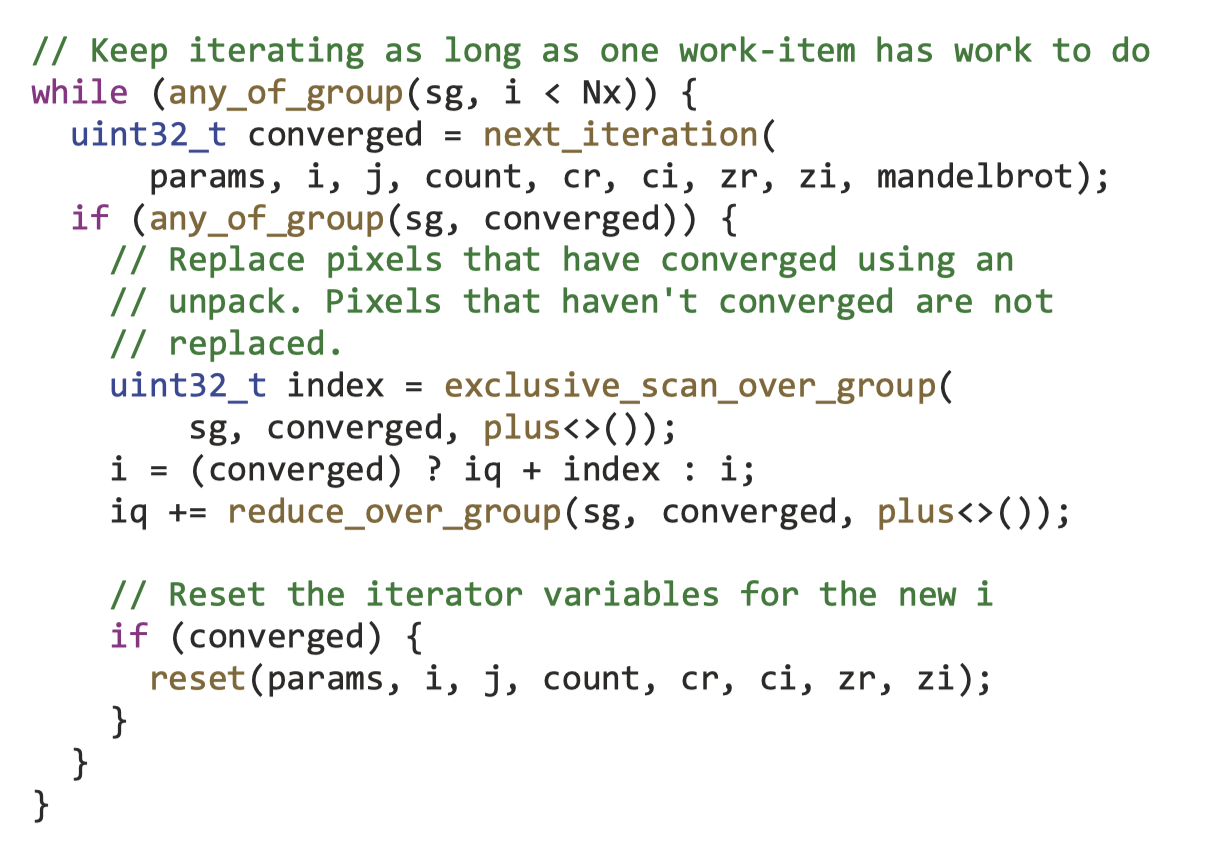
\includegraphics[width=0.9\textwidth]{figs/F14.26.png}
	\caption{\textit{使用Sub-Groups解包操作来改进具有不同控制流的Kernel的负载平衡 }}
\end{figure}

与 pack 一样,我们可以使用 scan 来实现 unpack。 图 14-25 显示了如何在独占扫描之上实现Sub-Groups解包操作。

图 14-26 中的代码演示了如何使用这样的Sub-Groups解包操作来改善具有发散控制流的Kernel中的负载平衡
(在本例中,计算 Mandelbrot 集)。 每个Work-Items都分配有一个单独的像素来计算和迭代,直到收敛或达到最大迭代次数。 
然后使用解包操作来用新像素替换完成的像素。

这种方法提高效率(并减少执行时间)的程度高度依赖于应用程序和输入,因为检查完成情况和执行解包操作都会带来一些开销! 
因此,在实际应用中成功使用此模式将需要根据存在的发散量和正在执行的计算进行一些微调
(例如,仅当活动Work-Items的数量低于某个阈值时才引入启发式方法来执行解包操作) )。

\subsection{总结}
本章演示了如何使用 SYCL 功能(包括内置函数和库)实现一些最常见的并行模式。

SYCL 生态系统仍在发展中,随着开发人员从该语言以及生产级应用程序和库的开发中获得更多经验,
我们期望为这些模式发现新的最佳实践。

\subsubsection{了解更多信息}
• 结构化并行编程:高效计算模式,作者:Michael McCool、Arch Robison 
和 James Reinders,© 2012,Morgan Kaufmann 出版,ISBN 978-0-124-15993-8。

• 算法库,C++ 参考,https://en.cppreference.com/w/cpp/algorithm。